\documentclass{article}

\usepackage[utf8]{inputenc}
\usepackage[T1]{fontenc} % Fixes font encoding
\usepackage{lmodern}     % Provides a scalable font for microtype to use

% --- newly added packages to fix current and future errors ---
\usepackage{graphicx}  % Fixes the \includegraphics error
\usepackage{xurl}      % Fixes the Overfull \hbox by allowing URLs to break anywhere
\usepackage{xcolor}    % Required for soul to do highlighting (\hl)
\usepackage{soul}      % Fixes the \ul (underline) and \hl (highlight) commands
\usepackage{longtable} % Fixes the longtable environment used later in the document
\usepackage{booktabs}  % Fixes the \toprule, \midrule, \bottomrule in your tables
\usepackage{array}     % Fixes \arraybackslash in your table columns
\usepackage{calc}      % Fixes the \real math used in your table column widths
\usepackage{textcomp}  % Ensures \textquotesingle renders correctly
\usepackage{microtype} % MAGIC BULLET: Fixes text justification and Overfull \hbox issues
% -------------------------------------------------------------

\usepackage{hyperref}  % Keep this loaded last!

\title{Research Assistant Task - Week 4}

\begin{document}
\maketitle
\section{Sample Selection}\label{sample-selection}

To align with the move toward a rule-based sample selection strategy for
next week, we will implement a sample selection methodology leveraging
1) the Geographical Segments in regulatory filings and 2) statistically
significant exposure to the orthogonal China factor. We were able to
find out the 1320 individual stock names for the MSCI World Index
components.

The Geographical Segments in regulatory filings are used to implement
selection filters. The Geographical Segments section is important
because we are trying to look at the impact on companies' exposure to
China, and this section likely provides the most telling information in
regards Chinese exposure since any significant geographical region needs
to be disclosed by law. The Geographical Segments section that companies
publicly report provide a verifiable revenue breakdown, allowing us a
glimpse into how much a firm is financially exposed in China and
provides a criteria for sample selection. However, we understand this
approach can have drawbacks as it can be skewed towards companies that
provide regulatory filings to the SEC based in US, meaning that this
approach could favor US and European companies.

To remove any platform bias, we also draw inspiration from the famed
Fama-French factor model. The Fama-French Three-Factor Model is a widely
used asset pricing model that extends traditional market risk by
incorporating additional factors: Size (SMB) and Value (HML). It breaks
down a stock\textquotesingle s expected return by its sensitivity to
these three factors, reflecting the empirical observation that smaller
companies and value stocks tend to generate higher long-term returns. We
take a step further and add Momentum (WML) and incorporate the Carhart
model, mainly because China tends to be very momentum driven.
Thereafter, exposure to the orthogonal China factor was investigated to
confirm that a company\textquotesingle s stock movements were being
systematically affected by a China-related risk, rather than broader
market forces. By isolating China influence, this selection criteria
ensures that a company stock movements are genuinely and systematically
exposed only to a measurable China-specific risk, rather than general
market turbulence.

\subsection{10\% Threshold in 10-K/20-F Geographical Segments}\label{threshold-in-10-k20-f-geographical-segments}

As a rule of thumb, FASB ASC 280 legally requires materiality threshold
for financial segment reporting under FASB guidelines, requiring
disclosure if a segment\textquotesingle s revenue, profit, or assets
meet or exceed 10\% of the company total. This standard is strictly
enforced by regulators and widely adopted by academic researchers
because it defines what geographic revenue data is legally material and
available for public analysis. Therefore, we could also use the 10\%
guideline to determine whether a company has ``significant'' exposure to
China or not in accordance with the FASB rule.

We have parsed the 10-Ks and 20-Fs of 1320 names that are shown in the
MSCI World index using Overseas Project Week4: EDGAR-MSCI World.ipynb.
Given this requires crawling through 10 years of reports for 1320 names,
a single pass is time-consuming (runs 10+ hours on Google Colab).

Using the threshold of 10\%, if a company has breached this threshold
within the 10 years between 2014-2025, then we blindly include it in the
universe regardless of what kind of sector the company is in.

There are 61 companies (removing the Chinese names JD, BABA, CLPS, DD,
SVA) that are filtered. The exposure trendlines for each companies can
be seen at 
\url{https://bychoix.github.io/overseas-project-week-4/china_revenue_proportion_chart.html}

Manually sifting through the individual companies, we can see that some
have pulled out of China operations BBY (Bestbuy) whereas ARE
(Alexandria Real Estate Equities) has revenue from China for 1 year in
2017 from sales of assets. On the other hand, this method does flag some
companies that were missed by our previous method such as VRSN
(Verisign), a tech company that is rarely mentioned in news articles
about trade tensions.

\vspace{0.5cm}
\noindent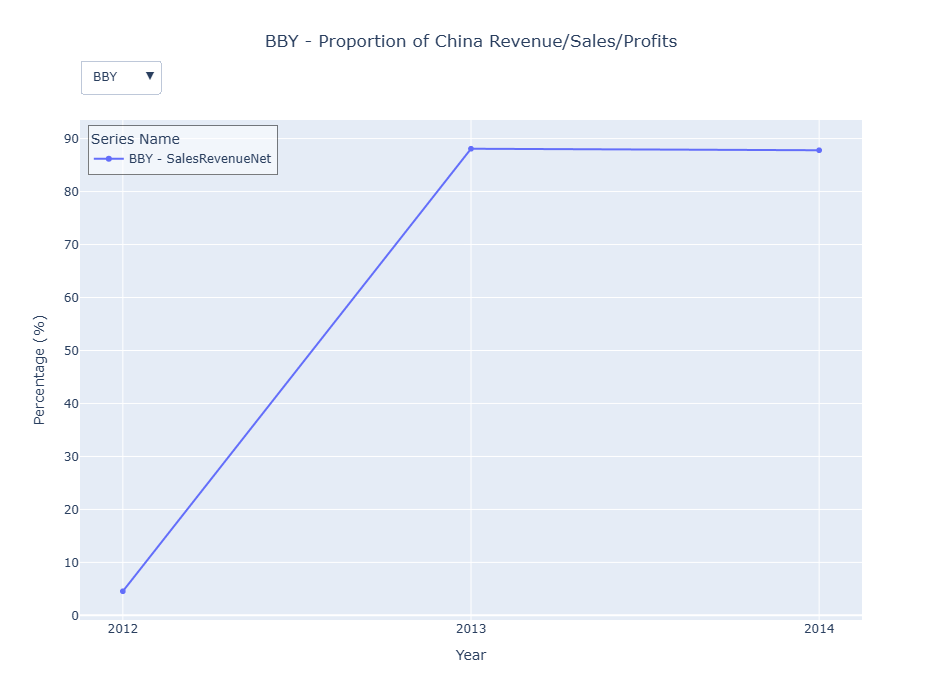
\includegraphics[width=0.48\textwidth]{images/media/image2.png}\hfill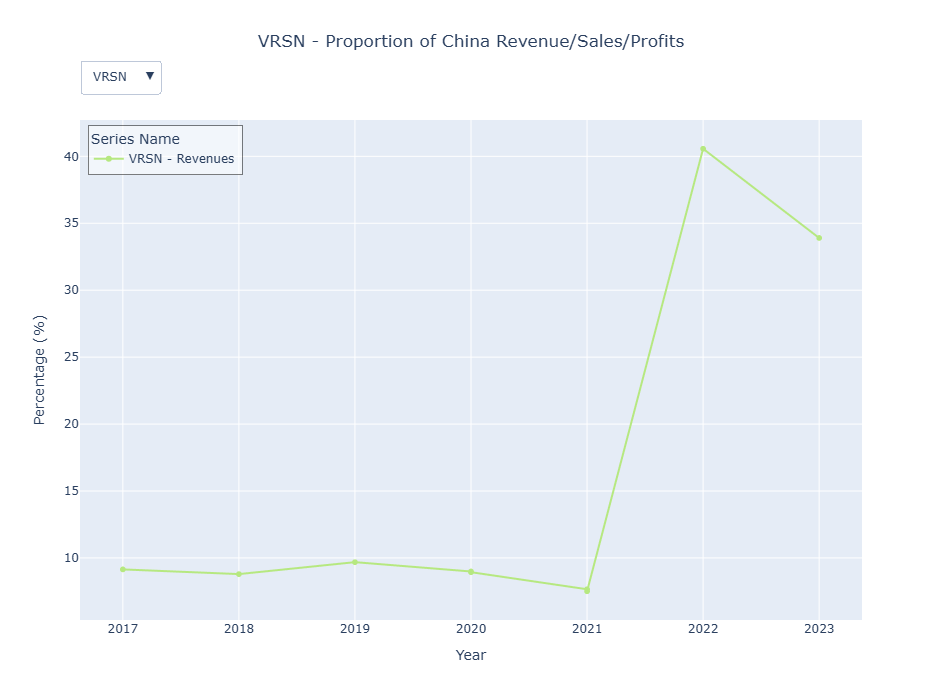
\includegraphics[width=0.48\textwidth]{images/media/image5.png}
\vspace{0.5cm}


\subsection{China Factor Exposure}\label{china-factor-exposure}

The Fama-French Three-Factor Model is a widely used asset pricing model
that extends traditional market risk by incorporating additional
factors: Size (SMB) and Value (HML). It posits that a
stock\textquotesingle s expected return is determined by its sensitivity
to these three factors, reflecting the empirical observation that
smaller companies and value stocks tend to generate higher long-term
returns. On top of the 3 factors already outlined by the Fama-French 3
factor model, we introduce another factor for China (China\_Orthogonal)
which orthogonalizes the MSCI China index price moves from the other
factors. From 2014 to 2025, we use the daily Fama-French 3 model from
Ken French's online library and we download the daily prices from Yahoo
finance for the stocks.

From the correlation matrix, we confirm that the China\_Orthogonal
factor that we introduce is fairly independent from the other factors,
which justifies the use of our new China factor. This is, in fact, by
design, as we have actually orthogonalized this factor whereas the other
factors are simply downloaded from the Fama-French database and does not
necessarily seem to be independent of one another.

\vspace{0.5cm}
\noindent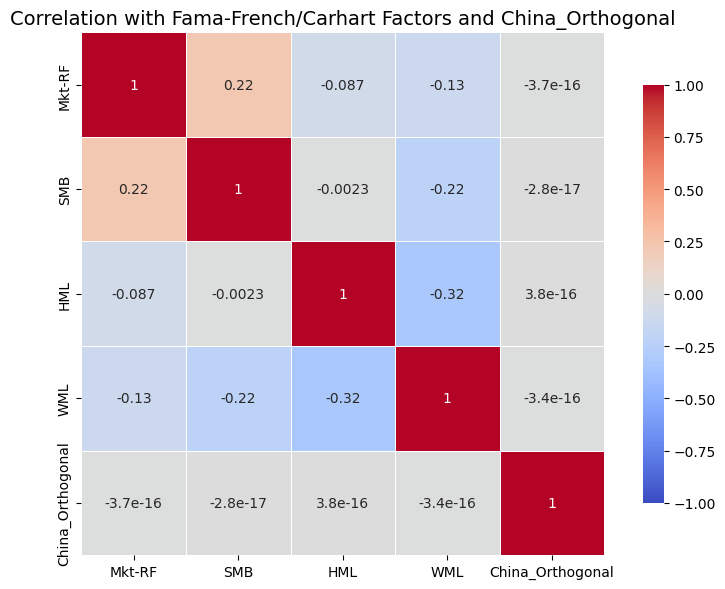
\includegraphics[width=\textwidth,keepaspectratio]{images/media/image3.png}
\vspace{0.5cm}

To ensure the China Factor Exposure is not a false discovery resulting
from data mining, we will use a stringent statistical threshold.
Following the findings of \emph{\ldots{} and the Cross-Section of
Expected Returns} (Harvey, Liu, and Zhu, 2016), we require a high bar
for statistically significant exposure" specifically requiring a
$t$-statistic of 3.0 or greater ($p$-value of 0.0027 or less) as even a
$t$-statistic of 2 can be considered noise from economic interpretation.
This elevated threshold moves beyond mere statistical significance to
ensure the factor\textquotesingle s impact is also economically
meaningful and strong enough to warrant inclusion in our final sample
selection. This filters down the 1320 names to 373 names (also
accounting for Chinese and Hong Kong names, which by default would be
highly correlated to the China factor), but this is still a large pool
to work with.

\emph{How many factors?} (Lewellen, 2022) further allows us to
distinguish when a factor is relevant by looking at the $R^2$ improvement.
In line with traditional academic emphasis on keeping asset-pricing
models parsimonious, it argues that for common applicationsoften
provides greater benefits by improving the model\textquotesingle s
overall statistical accuracy. The resulting increase in $R^2$ vindicates
the factor addition because it demonstrates that the new factor
successfully absorbs residual variation in stock returns.

When adding a factor to these factor models, $R^2$ never decreases
(Wooldridge Chapter 4, 2006). As this is the case, we add another filter
on top of an 1\% increase in $R^2$, by using AIC to confirm the model fit.
As a rule of thumb, an AIC improvement of 10 or greater allows us to
dismiss the previous model and elect the new model as the better fit
(Burnham and Anderson Chapter 2, 2002).

\begin{flushleft}
Hence, by using thresholds of $\Delta R^2 > 1\%$ and $\Delta AIC > 10$, we are left with 48 names (filtering out Chinese
companies): \textquotesingle BHP\textquotesingle,
\textquotesingle SCCO\textquotesingle,
\textquotesingle LVS\textquotesingle,
\textquotesingle HSBC\textquotesingle,
\textquotesingle MT\textquotesingle,
\textquotesingle TECK\textquotesingle,
\textquotesingle FCX\textquotesingle,
\textquotesingle BMWKY\textquotesingle,
\textquotesingle TTE\textquotesingle,
\textquotesingle IFNNY\textquotesingle,
\textquotesingle EQNR\textquotesingle,
\textquotesingle CHT\textquotesingle,
\textquotesingle WDS\textquotesingle,
\textquotesingle BP\textquotesingle,
\textquotesingle ING\textquotesingle,
\textquotesingle SAN\textquotesingle,
\textquotesingle E\textquotesingle,
\textquotesingle MBGAF\textquotesingle,
\textquotesingle STLA\textquotesingle,
\textquotesingle SONY\textquotesingle,
\textquotesingle MGA\textquotesingle,
\textquotesingle VIV\textquotesingle,
\textquotesingle STM\textquotesingle,
\textquotesingle BBVA\textquotesingle,
\textquotesingle SHEL\textquotesingle,
\textquotesingle PHG\textquotesingle,
\textquotesingle YARIY\textquotesingle,
\textquotesingle BUD\textquotesingle,
\textquotesingle JOF\textquotesingle,
\textquotesingle TS\textquotesingle,
\textquotesingle ASML\textquotesingle,
\textquotesingle POAHF\textquotesingle,
\textquotesingle ASX\textquotesingle,
\textquotesingle HMC\textquotesingle,
\textquotesingle MU\textquotesingle,
\textquotesingle IX\textquotesingle,
\textquotesingle RSG\textquotesingle,
\textquotesingle GRAB\textquotesingle,
\textquotesingle MELI\textquotesingle,
\textquotesingle NMR\textquotesingle,
\textquotesingle EL\textquotesingle,
\textquotesingle TM\textquotesingle,
\textquotesingle ENIC\textquotesingle,
\textquotesingle CMBT\textquotesingle,
\textquotesingle PPRUF\textquotesingle,
\textquotesingle EDPFY\textquotesingle,
\textquotesingle RIVN\textquotesingle,
\textquotesingle IE\textquotesingle{}
\end{flushleft}

\subsection{Finalized List of Companies}

To avoid selection bias, we implement a rule-based methodology to select
the pool of companies to be analyzed. We start with an unbiased universe
of 1320 names from the MSCI World index as a starting point. From there
we take a two-pronged approach: 1) using Geographical segments and
applying the universal 10\% cutoff for China exposure, and 2) using
price based criteria harnessing Fama-French/Carlhart factor models with
a China factor, and applying a threshold on the coefficient for the
China factor. The Geographical Segment approach yields 61 names and the
orthogonal Factor approach yields 48 names. Among these names there are
8 names that overlap \textquotesingle ASML\textquotesingle,
\textquotesingle FCX\textquotesingle,
\textquotesingle ING\textquotesingle,
\textquotesingle SONY\textquotesingle,
\textquotesingle PHG\textquotesingle,
\textquotesingle BHP\textquotesingle,
\textquotesingle MU\textquotesingle,
\textquotesingle EL\textquotesingle{} making a total of 101 names.

\vspace{0.5cm}
\noindent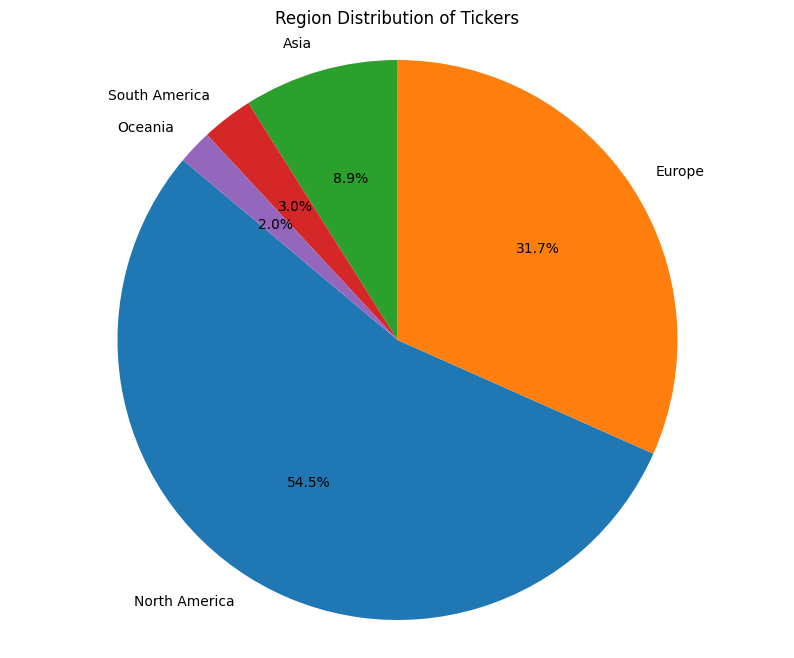
\includegraphics[width=0.48\textwidth]{images/media/image1.png}\hfill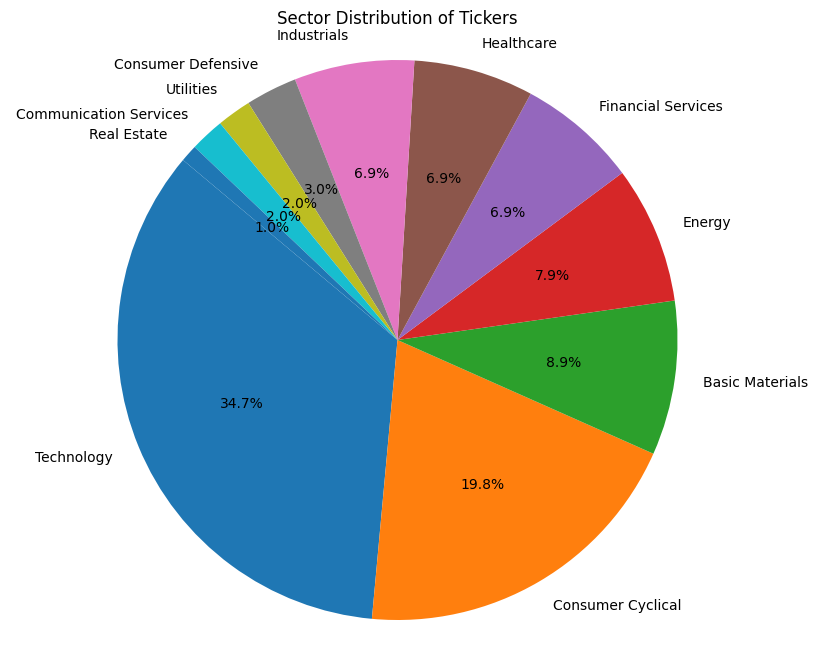
\includegraphics[width=0.48\textwidth]{images/media/image4.png}
\vspace{0.5cm}

\section{Dependent Variable Construction}\label{dependent-variable-construction}

\subsection{Strategy Classification and Category Definition}\label{strategy-classification-and-category-definition}

The dependent variable is constructed as a three-category firm-year
strategic classification: Retrenchment, Maintain, and Double Down.
Following the strategic restructuring literature, particularly Bowman
and Singh (1993), we treat corporate restructuring as a multidimensional
process rather than a one-directional strategic move. Bowman and Singh
explicitly characterize portfolio restructuring as a reconfiguration of
the firm's business mix through acquisitions and divestitures.
Consistent with this view, we define Retrenchment to include two cases:
(1) firm-years with exit signals only, and (2) firm-years with mixed
signals that contain both exit and expansion elements.

We classify mixed signals as Retrenchment for three reasons. First,
acquisitions and divestitures are often joint components of broader
corporate reconfiguration; accordingly, the coexistence of expansion and
exit signals is more consistent with strategic repositioning than with
pure expansion (Bowman \& Singh, 1993). Second, when political or
geopolitical risk rises, firms often retrench investment and employment
and adopt defensive responses. In this context, the coexistence of
expansion and exit signals under heightened uncertainty may reflect risk
management or option-preserving behavior rather than unequivocal
offensive expansion (Hassan et al., 2019). Third, the disclosure
literature suggests that managers communicate negative information
strategically and often accompany it with supplementary narrative
disclosures to shape investor interpretation. As a result, expansionary
language in mixed cases may not always correspond to substantive
commitment and may partly serve a rhetorical or cushioning function
(Skinner, 1994).

By contrast, Maintain is defined as firm-years with neither exit nor
expansion signals, capturing strategic inertia or status quo
positioning. Double Down captures firm-years with expansion signals
only, indicating a clear commitment to increasing China exposure.

This classification yields a relatively balanced distribution across
categories: Retrenchment (33.0\%), Maintain (32.6\%), and Double Down
(34.4\%). Such a distribution helps mitigate potential estimation issues
arising from class imbalance.

\subsection{External Validation of the Text-Based Strategy Measure}\label{external-validation-of-the-text-based-strategy-measure}

To address the concern that the text-based strategy measure may capture
disclosure language rather than underlying strategic behavior, we
conduct an external validation test following the logic of Bozanic,
Roulstone, and Van Buskirk (2018). In their study, forward-looking
statements are classified along two dimensions---whether the statement
is earnings-related and whether it is quantitative---and the validity of
this classification is assessed by testing whether these text attributes
predict the existence of management forecasts recorded in the I/B/E/S
guidance dataset. They also supplement this approach with a small-sample
manual audit of forecast records.

Adapting this logic to our setting, we use subsequent China revenue
outcomes as an external benchmark for our text-based China strategy
classification. If the measure captures meaningful strategic positioning
rather than merely rhetorical disclosure, firm-years classified as
Double Down should exhibit stronger subsequent China revenue growth than
those classified as Retrenchment, with Maintain expected to lie in
between.

We compute the change in China revenue ratio (China Revenue / Total
Sales) from year $t$ to $t+1$ for all firm-years with valid data. Table 1
Panel A shows that mean changes are monotonically ordered as predicted:
Retrenchment firms experience an average decline of 0.35 percentage
points, Maintain firms decline 0.16 percentage points, and Double Down
firms increase 0.72 percentage points.

\begin{table}[htbp]
\centering
\caption{External Validation of Text-Based Strategy Measure}
\vspace{0.2cm}

\textbf{Panel A: Descriptive Statistics by Strategy Category}
\vspace{0.1cm}

\begin{tabular}{lccc}
\toprule
 & \multicolumn{3}{c}{$\Delta$ China Revenue Ratio ($t \rightarrow t+1$)} \\
\cmidrule(lr){2-4}
Strategy ($t$) & Mean & Std. Dev. & Median \\
\midrule
Retrenchment & -0.0035 & 0.0524 & -0.0012 \\
Maintain     & -0.0016 & 0.0583 &  0.0009 \\
Double Down  &  0.0072 & 0.0395 &  0.0021 \\
\midrule
Difference (DD - Retrench) & 0.0107 & & 0.0033 \\
\bottomrule
\end{tabular}

\vspace{0.5cm}

\textbf{Panel B: Regression and Robustness Tests}
\vspace{0.1cm}

\begin{tabular}{llcc}
\toprule
Test & Statistic & $p$-value & Sig. \\
\midrule
OLS Regression (clustered SE) & $\beta = 0.0054$ & 0.019 & ** \\
OLS with Controls & $\beta = 0.0048$ & 0.026 & ** \\
One-sided T-test (DD $>$ Retrench) & $t = 1.48$ & 0.070 & * \\
Bootstrap (one-sided) & diff = 0.0107 & 0.069 & * \\
Cohen's $d$ Effect Size & $d = 0.230$ & -- & -- \\
\bottomrule
\multicolumn{4}{p{10cm}}{\footnotesize \textit{Notes:} *** $p<0.01$, ** $p<0.05$, * $p<0.10$. One-sided tests reflect the directional hypothesis that Double Down firms exhibit higher subsequent China revenue growth than Retrenchment firms. Standard errors in OLS regressions are clustered by firm.}
\end{tabular}
\end{table}

Panel B reports regression results where Strategy\_DV is coded as $-$1
(Retrenchment), 0 (Maintain), +1 (Double Down). The coefficient is
positive and significant ($\beta = 0.0054$, $p = 0.019$), indicating that a
one-unit increase in strategy classification is associated with a 0.54
percentage point increase in subsequent China revenue ratio. Results
remain robust with controls ($\beta = 0.0048$, $p = 0.026$). Supplementary
one-sided tests are marginally significant at the 10\% level ($t$-test $p = 0.070$; bootstrap $p = 0.068$).

Overall, the evidence suggests that the measure is not merely rhetorical
disclosure language, but is meaningfully related to subsequent realized
China revenue outcomes.

\newpage
\section{Independent Variable Construction}\label{independent-variable-construction}

\subsection{Method Reference}\label{method-reference}

Recent research highlights FinBERT\textquotesingle s ability to extract
sentiment information that goes beyond what is found in raw financial
figures. \emph{Extracting the Structure of Press Releases for Predicting
Earnings Announcement Returns} (Wu, et al, 2025) demonstrates that
FinBERT can actually outperform traditional "earnings surprises" in
terms of feature importance for predicting market returns. Using SHAP
(Shapley Additive Explanations) to measure the impact of different
variables, the study found the following distribution of predictive
importance that underscores that the qualitative "soft information"
captured by FinBERT provides a more significant signal for predicting
announcement returns.

\subsection{Contextual Appropriateness}\label{contextual-appropriateness}

Based on the findings of \emph{Fine-Tuning and Explaining FinBERT
for Sector-Specific Financial News: A Reproducible Workflow} (Cristescu,
2025), fine-tuning on a gold-standard corpus of 1,500 sector-tagged
headlines raised the macro F1-score from 0.555 (zero-shot) to 0.707
(few-shot fine-tuned), whereas Loughran-McDonald only achieves 0.482
F1-score. Additionally the fine-tuned model achieved an improved
accuracy of 71.6\%.

\section{Control Variables}\label{control-variables}

To isolate the relationship between Executive China Sentiment and firms'
subsequent China strategy choices, we include a set of control variables
at the firm, industry, macro, and China-exposure levels. These variables
are intended to account for observable factors that may independently
shape firms' strategic decisions and, at the same time, correlate with
managerial communication.

\subsection{Firm-level controls}\label{firm-level-controls}

We control for firm size, as larger firms typically possess greater
organizational resources, broader international operating capacity, and
stronger ability to absorb geopolitical risk. Prior research shows that
firms\textquotesingle{} cross-border entry and geographic allocation
decisions are shaped by both environmental uncertainty and
organizational capabilities, making size a relevant proxy for strategic
capacity (Henisz and Delios, 2001).

We also control for leverage, since financial obligations may constrain
firms\textquotesingle{} flexibility in maintaining overseas commitments
or undertaking expansion. More highly leveraged firms may be more likely
to retrench or adjust international operations under uncertainty, making
leverage an important control in models of foreign strategic adjustment
(Berry, 2013; Bergh, 1997).

Profitability (ROA) is included because better-performing firms
generally have greater internal capacity to expand, whereas
weaker-performing firms are more likely to refocus, restructure, or
retrench. Prior studies link firm performance to divestiture,
refocusing, and broader restructuring behavior, suggesting that
profitability is a standard and theoretically grounded control (Lee and
Madhavan, 2010; Markides, 1992).

Finally, we control for the cash ratio, which captures liquidity buffers
and strategic flexibility. Firms with stronger cash positions are better
able to absorb uncertainty, delay irreversible decisions, or expand when
opportunities arise, while financially constrained firms may be more
likely to contract. This logic is consistent with evidence on cash
holdings, financial constraints, and precautionary motives (Denis and
Sibilkov, 2010; Bates, Kahle, and Stulz, 2009).

All firm-level financial variables, including size, leverage, ROA, cash
ratio, are obtained from WRDS Compustat Capital IQ North America and
Global databases.

\subsection{ Industry-level controls} \label{industry-level-controls}

At the industry level, we control for industry China growth, which
captures time-varying market opportunities in China at the sector level.
If a given industry is growing rapidly in the Chinese market, firms in
that industry may be more likely to expand; if industry growth is weak,
firms may instead remain cautious or retrench. Industry China growth
therefore serves as a proxy for sector-specific demand conditions and
strategic opportunity in China (Henisz and Delios, 2001). This variable
is constructed from Chinese National Bureau of Statistics sales data.

We also include the Lerner Index as a measure of product market
competition. Industry competition affects firms\textquotesingle{}
pricing power, strategic discretion, and ability to deviate from
prevailing industry trends. Firms in less competitive industries,
reflected in higher Lerner values, may have greater room for independent
strategic action, whereas firms in highly competitive industries may be
more constrained by market pressure and peer behavior. The Lerner Index
is a widely used proxy for market power and competitive intensity in the
economics and finance literature (Aghion et al., 2005; Gaspar and Massa,
2006). This variable is measured as the annual average Lerner index of
China-related firms within each industry, calculated using CSMAR data.

\subsection{Macro-level controls}\label{macro-level-controls}

We control China GDP growth to capture macroeconomic conditions in the
Chinese market. Changes in China\textquotesingle s economic growth
directly affect the attractiveness, demand conditions, and expected
profitability of China-related operations. Stronger macroeconomic growth
may encourage expansion, whereas weaker growth may induce caution or
contraction. This variable is measured using World Bank data (series:
NY.GDP.MKTP.KD.ZG).

We further include the USD/CNY exchange rate, since exchange-rate
movements affect the relative profitability, cost structure, and risk
exposure of China-related activities. Exchange-rate fluctuations can
alter both the dollar value of China revenues and
firms\textquotesingle{} broader operating and hedging decisions, making
them a relevant macro-level determinant of strategy (Hoberg and Moon,
2017). Exchange rate volatility is constructed from FRED daily exchange
rate data.

In addition, we control for China Economic Policy Uncertainty (EPU), as
policy uncertainty may simultaneously shape firms\textquotesingle{}
strategic choices and managerial communication. Periods of heightened
policy or geopolitical tension may lead firms to delay investment,
reduce commitments, or adopt more cautious strategic positions, making
such uncertainty a common shock that must be accounted for empirically
(Baker, Bloom, and Davis, 2016; Caldara and Iacoviello, 2022). This
variable is measured using the FRED series CHNMAINLANDEPU, based on
Baker, Bloom, and Davis (2016), capturing uncertainty related to
regulation, trade policy, and industrial policy.

\subsection{China-exposure controls}\label{china-exposure-controls}

Finally, we control the firm\textquotesingle s China revenue ratio,
which captures its pre-existing commitment and exposure to the Chinese
market. Firms with greater China revenue dependence may have stronger
incentives to maintain or deepen their China presence because of sunk
costs, path dependence, and accumulated local knowledge; at the same
time, concentrated exposure may also increase pressure to retrench when
risk rises. Existing international business research suggests that prior
foreign commitment, subsidiary experience, and sequential investment
patterns are important determinants of subsequent strategic decisions,
making China revenue exposure a theoretically important control (Benito,
2005; Berry, 2013; Delios and Beamish, 2001; Chang and Rosenzweig,
2001).

\section{Estimation Models}\label{estimation-models}

A key identification challenge is the potential for reverse causality:
firms that have already decided on a particular China strategy may
express sentiment consistent with that predetermined decision. To
address this concern, we employ two strategies.

First, following Berry (2013), we use lagged independent variables,
measuring sentiment and all control variables in year $t-1$ to predict
strategic outcomes in year $t$. This temporal ordering ensures that the
sentiment measure precedes the observed strategic action, strengthening
our ability to make causal inferences. Second, following standard
practice in panel studies of corporate responses to policy uncertainty
(e.g., Hassan et al., 2019; Bloom et al., 2007), we include year fixed
effects to absorb time-varying macroeconomic shocks and policy changes
that may simultaneously affect both executive sentiment and strategic
decisions. When year fixed effects are included, macro-level controls
(e.g., policy tension) are excluded to avoid perfect collinearity, as
these factors are absorbed by the year dummies.

\begin{longtable}[]{@{}
  >{\raggedright\arraybackslash}p{(\linewidth - 12\tabcolsep) * \real{0.2532}}
  >{\centering\arraybackslash}p{(\linewidth - 12\tabcolsep) * \real{0.1177}}
  >{\centering\arraybackslash}p{(\linewidth - 12\tabcolsep) * \real{0.1177}}
  >{\centering\arraybackslash}p{(\linewidth - 12\tabcolsep) * \real{0.1161}}
  >{\centering\arraybackslash}p{(\linewidth - 12\tabcolsep) * \real{0.1161}}
  >{\centering\arraybackslash}p{(\linewidth - 12\tabcolsep) * \real{0.1177}}
  >{\centering\arraybackslash}p{(\linewidth - 12\tabcolsep) * \real{0.1161}}@{}}
\toprule
 & \multicolumn{5}{c}{Ordered Logit} & OLS \\
\cmidrule(lr){2-6} \cmidrule(lr){7-7}
 & (1) & (2) & (3) & (4) & (5) & (6) \\
\midrule
\endfirsthead
\toprule
 & \multicolumn{5}{c}{Ordered Logit} & OLS \\
\cmidrule(lr){2-6} \cmidrule(lr){7-7}
 & (1) & (2) & (3) & (4) & (5) & (6) \\
\midrule
\endhead
Executive China Sentiment t-1 & 0.544** & 0.506** & 0.537** & 0.527** & 0.523** & 0.237** \\
 & (2.40) & (2.19) & (2.31) & (2.27) & (2.20) & (2.27) \\
Firm Controls & & Yes & Yes & Yes & Yes & Yes \\
Industry Controls & & & Yes & Yes & Yes & Yes \\
Macro Controls & & & & Yes & & \\
Year FE & & & & & Yes & Yes \\
Pseudo $R^2$ / $R^2$ & 0.005 & 0.009 & 0.010 & 0.011 & 0.017 & 0.037 \\
\bottomrule
\end{longtable}


\section{Measurement Robustness}\label{measurement-robustness}

We further examine whether our findings are sensitive to how executive
China sentiment is operationalized. In addition to the baseline
measure---the mean FinBERT sentiment score---we test four alternative
specifications: positive tone share, negative tone share, net sentiment
(positive minus negative), and the sentiment ratio (the share of
positive tone relative to total sentiment expressions).

The results indicate strong measurement robustness. All five sentiment
measures exhibit the theoretically expected sign: positive sentiment
measures are positively associated with subsequent double-down
strategies, whereas negative tone share is negatively associated with
such outcomes. Three of the five measures are statistically significant
at conventional levels.

Notably, negative tone share produces the largest and most statistically
significant effect ($\beta = -1.148$, $z = -2.64$, $p = 0.008$), suggesting
that expressions of concern or pessimism about China are especially
predictive of subsequent retrenchment decisions. This pattern is
consistent with prospect theory (Kahneman and Tversky, 1979), which
argues that negative information tends to weigh more heavily in
decision-making than equivalent positive information.

Overall, the consistency across alternative sentiment measures---with
all specifications showing the expected sign direction and a majority
reaching statistical significance---suggests that the main result is not
driven by a particular measurement choice. Instead, it appears to
reflect a robust underlying relationship between executive sentiment
toward China and subsequent strategic action.


\begin{longtable}[]{@{}
  >{\raggedright\arraybackslash}p{(\linewidth - 10\tabcolsep) * \real{0.1837}}
  >{\centering\arraybackslash}p{(\linewidth - 10\tabcolsep) * \real{0.1660}}
  >{\centering\arraybackslash}p{(\linewidth - 10\tabcolsep) * \real{0.1337}}
  >{\centering\arraybackslash}p{(\linewidth - 10\tabcolsep) * \real{0.1418}}
  >{\centering\arraybackslash}p{(\linewidth - 10\tabcolsep) * \real{0.1643}}
  >{\centering\arraybackslash}p{(\linewidth - 10\tabcolsep) * \real{0.1676}}@{}}
\toprule
\textbf{Variable} & \textbf{Mean Sentiment (Baseline)} & \textbf{Positive Tone Share} & \textbf{Negative Tone Share} & \textbf{Net Sentiment (Pos $-$ Neg)} & \textbf{Sentiment Ratio (Pos / Total)} \\
\midrule
\endfirsthead
\toprule
\textbf{Variable} & \textbf{Mean Sentiment (Baseline)} & \textbf{Positive Tone Share} & \textbf{Negative Tone Share} & \textbf{Net Sentiment (Pos $-$ Neg)} & \textbf{Sentiment Ratio (Pos / Total)} \\
\midrule
\endhead
\textbf{Sentiment Measure} & 0.537** & 0.412 & -1.148*** & 0.537** & 0.317 \\
\textbf{z-statistic} & (2.31) & (1.26) & (-2.64) & (2.31) & (1.32) \\
\textbf{Expected Sign} & (+) & (+) & (-) & (+) & (+) \\
\textbf{Firm Controls} & Yes & Yes & Yes & Yes & Yes \\
\textbf{Industry Controls} & Yes & Yes & Yes & Yes & Yes \\
\bottomrule
\end{longtable}

\noindent{\footnotesize\textit{Notes:} Ordered Logit estimates. DV: Strategy coded as -1 (Retrenchment), 0 (Maintain), +1 (Double Down). All independent variables lagged by one year. z-statistics in parentheses. Expected signs: Positive/Net/Ratio measures should have (+) coefficients; Negative tone should have (-). *** $p<0.01$, ** $p<0.05$, * $p<0.10$.}

\section{Additional Robustness Analysis}\label{additional-robustness-analysis}

To examine whether the relationship between executive sentiment and
China strategy varies across time periods and industries, we conduct
subsample analyses.

We divide the sample around two major structural breaks: the onset of
the U.S.--China trade tensions in 2018 and the COVID-19 pandemic in
2020. Although the coefficient estimates remain positive across all
subsamples, ranging from 0.250 to 0.515, statistical significance
appears only in the post--trade war period ($\beta = 0.515$, $p = 0.055$).
This pattern likely reflects reduced statistical power in the smaller
subsamples rather than a substantive change in the underlying
relationship. Consistent with this interpretation, the interaction terms
for Sentiment $\times$ Post-Trade War and Sentiment $\times$ Post-COVID are both
statistically insignificant ($p = 0.744$ and $p = 0.970$, respectively),
suggesting that the sentiment--strategy relationship is broadly stable
over time rather than driven by a particular period.

In different industries, the estimated coefficient is largest in the
Automotive sector ($\beta = 0.896$) and smallest in Pharmaceuticals ($\beta = 0.253$), with Information Technology lying in between ($\beta = 0.625$, $p = 0.062$). However, the interaction model provides no evidence of
statistically significant industry heterogeneity: neither Sentiment $\times$
Pharma nor Sentiment $\times$ Auto is significant ($p = 0.577$ and $p = 0.361$,
respectively). This suggests that the main effect is not driven
disproportionately by any single industry.

\section{Endogeneity Concerns}\label{endogeneity-concerns}

We conduct several tests to assess potential endogeneity concerns
related to omitted variables and reverse causality.

Our baseline model uses lagged sentiment ($t-1$) to predict current
strategy ($t$), which helps establish temporal ordering. However,
additional tests suggest a more dynamic relationship. In a Granger-style
specification controlling for lagged strategy, lagged sentiment remains
positive but becomes statistically insignificant ($\beta = 0.115$, $p = 0.159$), while lagged strategy significantly predicts current sentiment
($\beta = 0.059$, $p = 0.008$). A placebo-style test using future sentiment
($t+1$) to predict current strategy also yields a significant coefficient
($\beta = 0.338$, $p = 0.006$), suggesting persistence in both strategy and
executive communication rather than a clean one-way causal effect.

We use two additional approaches to address endogeneity concerns:
Propensity Score Matching (PSM) and Generalized Method of Moments (GMM).

Propensity Score Matching. To mitigate selection on observables, we
match firms with high executive China sentiment (above the median) to
firms with low sentiment based on firm size, leverage, ROA, cash ratio,
industry China growth, and the Lerner index. Using nearest-neighbor
matching with a caliper of 0.1, we obtain 223 matched pairs.
Post-matching balance is satisfactory across all six covariates, with
standardized differences below 0.1. The estimated average treatment
effect on the treated (ATT) is 0.161 ($t=2.09$, $p=0.037$), indicating that
high-sentiment firms exhibit significantly higher subsequent strategy
scores than otherwise similar low-sentiment firms.

GMM Estimation. To address potential dynamic panel bias, we estimate
both Difference GMM and System GMM models. In both specifications, the
coefficient on sentiment remains positive (0.013 and 0.422,
respectively), although neither estimate is statistically significant.
This likely reflects limited statistical power given the relatively
small panel size. At the same time, the direction of the coefficients
remains consistent with the baseline findings, and the strong
persistence of strategy ($\beta = 0.358$, $p<0.001$)
supports the relevance of a dynamic specification.

Overall, the PSM results suggest that the sentiment--strategy
relationship is not solely driven by observable selection, while the GMM
estimates, though imprecise, remain directionally consistent with the
baseline results.

\section{Next Week}\label{next-week}

Next week we will focus on further expanding the dataset. For this
iteration, we will keep the sample selection primarily based on 10-K, as
these provide the cleanest and most feasible source at this stage. As a
possible future extension, we note the potential to incorporate
quarterly earnings call transcripts to enrich the executive sentiment
measure once the baseline sample construction is settled. We will then
re-estimate the main models on the expanded sample to assess the
robustness of our findings.

Furthermore, this would hinge upon whether we can finalize the company
universe we want to work with.

\newpage

\textbf{References}

Aghion, P., Bloom, N., Blundell, R., Griffith, R., \& Howitt, P. (2005).
Competition and innovation: An inverted-U relationship. \emph{Quarterly
Journal of Economics, 120}(2), 701--728.

Baker, S. R., Bloom, N., \& Davis, S. J. (2016). Measuring economic
policy uncertainty. \emph{Quarterly Journal of Economics, 131}(4),
1593--1636.

Bates, T. W., Kahle, K. M., \& Stulz, R. M. (2009). Why do U.S. firms
hold so much more cash than they used to? \emph{Journal of Finance,
64}(5), 1985--2021.

Benito, G. R. G. (2005). Divestment and international business strategy.
\emph{Journal of Economic Geography, 5}(2), 235--251.

Bergh, D. D. (1997). Predicting divestiture of unrelated acquisitions:
An integrative model of ex ante conditions. \emph{Strategic Management
Journal, 18}(9), 715--731.

Berry, H. (2013). When do firms divest foreign operations?
\emph{Organization Science, 24}(1), 246--261.

Bozanic, Z., Roulstone, D. T., \& Van Buskirk, A. (2018). Management
earnings forecasts and other forward-looking statements. \emph{Journal
of Accounting and Economics, 65}(1), 1--20.

Bowman, E. H., \& Singh, H. (1993). Corporate restructuring:
Reconfiguring the firm. \emph{Strategic Management Journal, 14}(S1),
5--14.

Burnham, K. P., \& Anderson, D. R. (2002). Model selection and
multimodel inference: A practical information-theoretic approach (2nd
ed.). Springer-Verlag

Caldara, D., \& Iacoviello, M. (2022). Measuring geopolitical risk.
\emph{American Economic Review, 112}(4), 1194--1225.

Chang, S.-J., \& Rosenzweig, P. M. (2001). The choice of entry mode in
sequential foreign direct investment. \emph{Strategic Management
Journal, 22}(8), 747--776.

Cristescu, C. (2025). \emph{Fine-tuning and explaining FinBERT for
sector-specific financial news: A reproducible workflow}. Electronics,
14(23), 4680.

Delios, A., \& Beamish, P. W. (2001). Survival and profitability: The
roles of experience and intangible assets in foreign subsidiary
performance. \emph{Academy of Management Journal, 44}(5), 1028--1038.

Denis, D. J., \& Sibilkov, V. (2010). Financial constraints, investment,
and the value of cash holdings. \emph{Review of Financial Studies,
23}(1), 247--269.

French, Kenneth R. "Data Library: Fama/French Factors."
\href{https://mba.tuck.dartmouth.edu/pages/faculty/ken.french/Data_Library/f-f_factors.html}{Dartmouth Tuck School of Business}

Gaspar, J.-M., \& Massa, M. (2006). Idiosyncratic volatility and product
market competition. \emph{Journal of Business, 79}(6), 3125--3152.

Harvey, C. R., Liu, Y., \& Zhu, H. (2016). \ldots{} and the
cross-section of expected returns. \emph{Review of Financial Studies,
29}(1), 5--68.

Hassan, T. A., Hollander, S., van Lent, L., \& Tahoun, A. (2019).
Firm-level political risk: Measurement and effects. \emph{Quarterly
Journal of Economics, 134}(4), 2135--2202.

Henisz, W. J., \& Delios, A. (2001). Uncertainty, imitation, and plant
location: Japanese multinational corporations, 1990--1996.
\emph{Administrative Science Quarterly, 46}(3), 443--475.

Hoberg, G., \& Moon, S. K. (2017). Offshore activities and financial vs.
operational hedging. \emph{Journal of Financial Economics, 125}(2),
217--244.

Lee, D., \& Madhavan, R. (2010). Divestiture and firm performance: A
meta-analysis. \emph{Journal of Management, 36}(6), 1345--1371.

Lewellen, J. (2022). \emph{How many factors?} Working paper, Tuck School
of Business at Dartmouth.

Markides, C. C. (1992). Consequences of corporate refocusing: Ex ante
evidence. \emph{Academy of Management Journal, 35}(2), 398--412.

Skinner, D. J. (1994). Why firms voluntarily disclose bad news.
\emph{Journal of Accounting Research, 32}(1), 38--60.

Wu, X., et al. (2025). \emph{Extracting the structure of press releases
for predicting earnings announcement returns}. SSRN Working Paper.

Wu, Yuntao, Ege Mert Akin, Charles Martineau, Vincent Grégoire, and
Andreas Veneris. Extracting the Structure of Press Releases for
Predicting Earnings Announcement Returns, \emph{arXiv preprint
arXiv:2509.24254}

\end{document}